\section{Results} \label{sec:results}

\begin{table} [H]
	\caption{Mean Square Error and R$^2$-score presented for OLS, Ridge, Lasso and Ridge + gradient descent (RidgeGD), where noise was added to the data. The parameters used were $\lambda=1e-5$ (penalty), $\eta=1e-4$ (learning rate), $\text{niter}=1e5$ (number of iterations) and $\mathcal{N}(0, \sigma^2=0.1)$ (noise). See text for more information.}
	\begin{tabularx}{\textwidth}{l|XXX|XXX} \hline\hline
		\label{tab:franke_error}
		& \multicolumn{3}{c}{\textbf{MSE}}&\multicolumn{3}{c}{\textbf{R2}}\\ \hline
		&Self&K-fold&Scikit&Self&K-fold&Scikit\\ \hline \\
		OLS & 0.008494 & 0.009119 & 0.008494 & 0.9048 & 0.8956 & 0.9048 \\
		Ridge & 0.009128 & 0.009651 & 0.009128 & 0.8977 & 0.8895 & 0.8977 \\
		Lasso & 0.01439 & 0.01489 & 0.01555 & 0.8387 & 0.8296 & 0.8257 \\
		RidgeGD & 0.01451 & 0.01504 & 0.009128 & 0.8373 & 0.8280 & 0.8977 \\ \hline
	\end{tabularx}
\end{table}

\iffalse
\begin{figure} [H]%
	\centering
	\subfloat[Lambda vs. R2-score]{{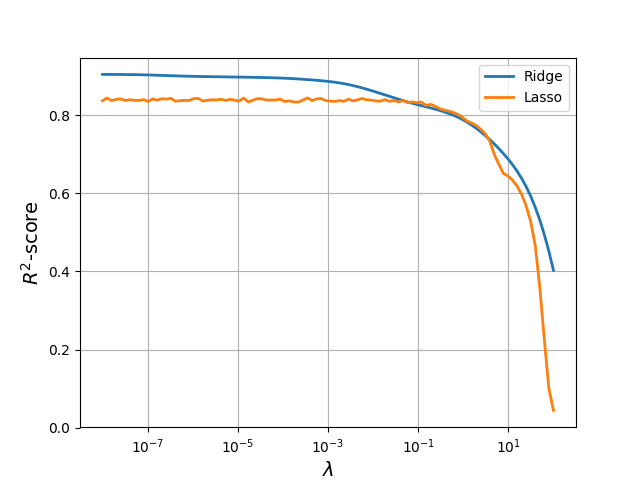
\includegraphics[width=7cm]{../plots/lambda_R2score.png} }}%
	\subfloat[Variance vs. R2-score]{{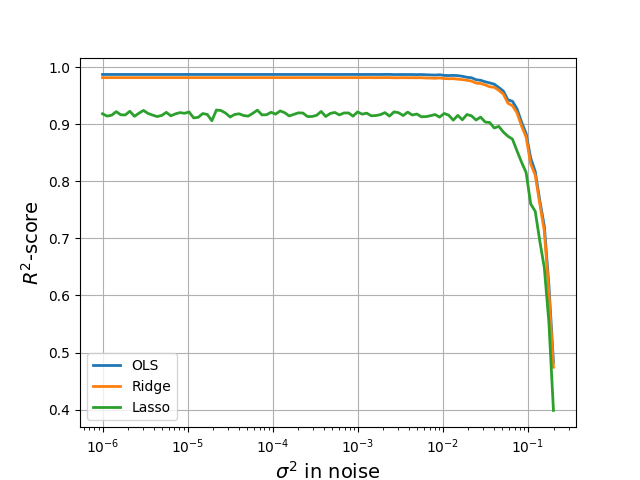
\includegraphics[width=7cm]{../plots/var_R2score.png} }}
	\caption{R$^2$-score plotted as a function of the penalty $\lambda$ (a) and as a function of the noise (b). $\lambda\in[10^{-8},10^2]$ in (a) and $\sigma^2\in[10^{-6},10^{-0.7}]$ in (b). The other parameters used were $\lambda=1e-5$ (penalty, was held constant for (b) only), $\eta=1e-4$ (learning rate), $niter=1e5$ (number of iterations) and $\mathcal{N}(0, \sigma^2=0.1)$ (noise, was held constant for (a) only).}%
	\label{fig:R2_scores}
\end{figure}
\fi 


